% -*- TeX-engine: xetex; eval: (auto-fill-mode 0); eval: (visual-line-mode 1); -*-
% Compile with XeLaTeX

%%%%%%%%%%%%%%%%%%%%%%%
% To do before class
%%%%%%%%%%%%%%%%%%%%%%%

% Send the Logistics/Week0Annoucnement (the night before).
% Send an email reminding students to bring a charged computer (the night before).

%%%%%%%%%%%%%%%%%%%%%%%
% Option 1: Slides: (comment for handouts)   %
%%%%%%%%%%%%%%%%%%%%%%%

\documentclass[slidestop,compress,mathserif,12pt,t,professionalfonts,xcolor=table]{beamer}

% solution stuff
\newcommand{\solnMult}[1]{
\only<1>{#1}
\only<2->{\red{\textbf{#1}}}
}
\newcommand{\soln}[1]{\textit{#1}}

\newcommand{\solnMultOn}[3]{
\only<#1>{#3}
\only<{#2}->{\red{\textbf{#3}}}
}

%%%%%%%%%%%%%%%%%%%%%%%%%%%%%%%
% Option 2: Handouts, without solutions (post before class)    %
%%%%%%%%%%%%%%%%%%%%%%%%%%%%%%%

% \documentclass[11pt,containsverbatim,handout,xcolor=xelatex,dvipsnames,table]{beamer}

% % handout layout
% \usepackage{pgfpages}
% \pgfpagesuselayout{4 on 1}[letterpaper,landscape,border shrink=5mm]

% % solution stuff
% \newcommand{\solnMult}[1]{#1}
% \newcommand{\soln}[1]{}
% \newcommand{\solnMultOn}[3]{#3}

% % % This breaks things for me for some reason.
% % tell pgfpages how to set page sizes in XeLaTeX
% %\renewcommand\pgfsetupphysicalpagesizes{%
% %   \pdfpagewidth\pgfphysicalwidth\pdfpageheight\pgfphysicalheight%
% %}

%%%%%%%%%%%%%%%%%%%%%%%%%%%%%%%%%%%%
% Option 3: Handouts, with solutions (may post after class if need be)    %
%%%%%%%%%%%%%%%%%%%%%%%%%%%%%%%%%%%%

% \documentclass[11pt,containsverbatim,handout,xcolor=xelatex,dvipsnames,table]{beamer}

% % handout layout
% \usepackage{pgfpages}
% \pgfpagesuselayout{4 on 1}[letterpaper,landscape,border shrink=5mm]

% % solution stuff
% \newcommand{\solnMult}[1]{\red{\textbf{#1}}}
% \newcommand{\soln}[1]{\textit{#1}}

% % % This breaks things for me for some reason.
% % % tell pgfpages how to set page sizes in XeLaTeX
% % \renewcommand\pgfsetupphysicalpagesizes{%
% %    \pdfpagewidth\pgfphysicalwidth\pdfpageheight\pgfphysicalheight%
% % }

%%%%%%%%%%%%%%%%%%%%%%%%%%%%%%%
% Option 4: Notes Only
%%%%%%%%%%%%%%%%%%%%%%%%%%%%%%%

% % See http://tex.stackexchange.com/questions/114219/add-notes-to-latex-beamer
% \documentclass[10pt,containsverbatim,xcolor=xelatex,dvipsnames,table,notes=only]{beamer}

% % handout layout
% % \usepackage{pgfpages}
% % \pgfpagesuselayout{1 on 1}[letterpaper, landscape, border shrink=5mm]

% % solution stuff
% \newcommand{\solnMult}[1]{#1}
% \newcommand{\soln}[1]{}

% % % Having a problem with this.
% % tell pgfpages how to set page sizes in XeLaTeX
% % \renewcommand\pgfsetupphysicalpagesizes{%
% %   \pdfpagewidth\pgfphysicalwidth\pdfpageheight\pgfphysicalheight%
% %}

%%%%%%%%%%
% Load style file, defaults  %
%%%%%%%%%%

\input{../../lec_style.tex}
% You cannot use numbers when defining variables.  Hence the use of letters, A, B, C, etc.

% Personal Info
\newcommand{\FirstName}{Mine}
\newcommand{\LastName}{\c{C}etinkaya-Rundel}
\newcommand{\OfficeHours}{MTWR 3-4pm.}
\newcommand{\OfficeHoursLocation}{Old Chem 213}

% Electronic Info
\newcommand{\PersonalSite}{http://stat.duke.edu/~mc301}
\newcommand{\CourseSite}{http://bitly.com/sta101sp15}
\newcommand{\Email}{mine@stat.duke.edu}

% TAs
\newcommand{\TAA}{Anthony Weishampel}
\newcommand{\TAB}{Fiamma Li}
\newcommand{\TAC}{Jialiang Mao}
\newcommand{\TAD}{Phillip Lee}

% Exam Dates
\newcommand{\ExamADate}{Wed, Feb 18}
\newcommand{\ExamBDate}{Wed, Mar 25}
\newcommand{\FinalDate}{Sat, May 2 (2-5pm)}

% Due Dates
\newcommand{\ClickerRegistrationDD}{Mon, Jan 26}
\newcommand{\GettingToKnowYouDD}{Friday, Jan 9, 11:59pm}
\newcommand{\ProblemSetADD}{Wed., 1/15}


% ALT ALT
%% You cannot use numbers when defining variables.  Hence the use of letters, A, B, C, etc.

% Personal Info
\renewcommand{\FirstName}{Jesse}
\renewcommand{\LastName}{Windle}
\renewcommand{\OfficeHours}{Tue, Thu 3:00pm-4:30pm}
\renewcommand{\OfficeHoursLocation}{Old Chem 211D}

% Electronic Info
\renewcommand{\PersonalSite}{http://stat.duke.edu/~jbw44/}
\renewcommand{\CourseSite}{http://bitly.com/windle2}
\renewcommand{\Email}{jbw44@stat.duke.edu}

% TAs
\renewcommand{\TAA}{David Clancy}
\renewcommand{\TAB}{Xinyi (Chris) Li}
\renewcommand{\TAC}{Tori Hall}
\renewcommand{\TAD}{Radhika Anand}

% Exam Dates
\renewcommand{\ExamADate}{Thu, Feb 19}
\renewcommand{\ExamBDate}{Thu, Mar 26}
\renewcommand{\FinalDate}{Mon, Apr 27 (9-Noon)}

% Due Dates
\renewcommand{\ClickerRegistrationDD}{Thu, Jan 15}
\renewcommand{\GettingToKnowYouDD}{Friday, Jan 9, 11:59pm}
\renewcommand{\ProblemSetADD}{Thu., 1/16}

%%%%%%%%%%%
% Cover slide info    %
%%%%%%%%%%%

\title{Unit 7: Multiple linear regression}
\subtitle{4. Transformations and case study}
\author{Sta 101 - Spring 2015}
\date{April 15, 2015}
\institute{Duke University, Department of Statistical Science}

%%%%%%%%%%%
% Begin document   %
%%%%%%%%%%%

\begin{document}

%%%%%%%%%%%%%%%%%%%%%%%%%%%%%%%%%%%%

% Title Page

\begin{frame}[plain]

\titlepage
\vfill
{\scriptsize \webLink{\PersonalSite}{Dr. \LastName{}} \hfill Slides posted at  \webLink{\CourseSite}{\CourseSite}}
\addtocounter{framenumber}{-1} 

\end{frame}

%%%%%%%%%%%%%%%%%%%%%%%%%%%%%%%%%%%%

\section{Housekeeping}

%%%%%%%%%%%%%%%%%%%%%%%%%%%%%%%%%%%%

\begin{frame}
\frametitle{Announcements}

\begin{itemize}

\item 

\end{itemize}

\end{frame}

%%%%%%%%%%%%%%%%%%%%%%%%%%%%%%%%%%%%

\section{Transformations}

%%%%%%%%%%%%%%%%%%%%%%%%%%%%%%%%%%%%

\begin{frame}[fragile]
\frametitle{Truck prices}

\disc{The scatterplot below shows the relationship between year and price of a random sample of 43 pickup trucks. Describe the relationship between these two variables.}

\begin{center}
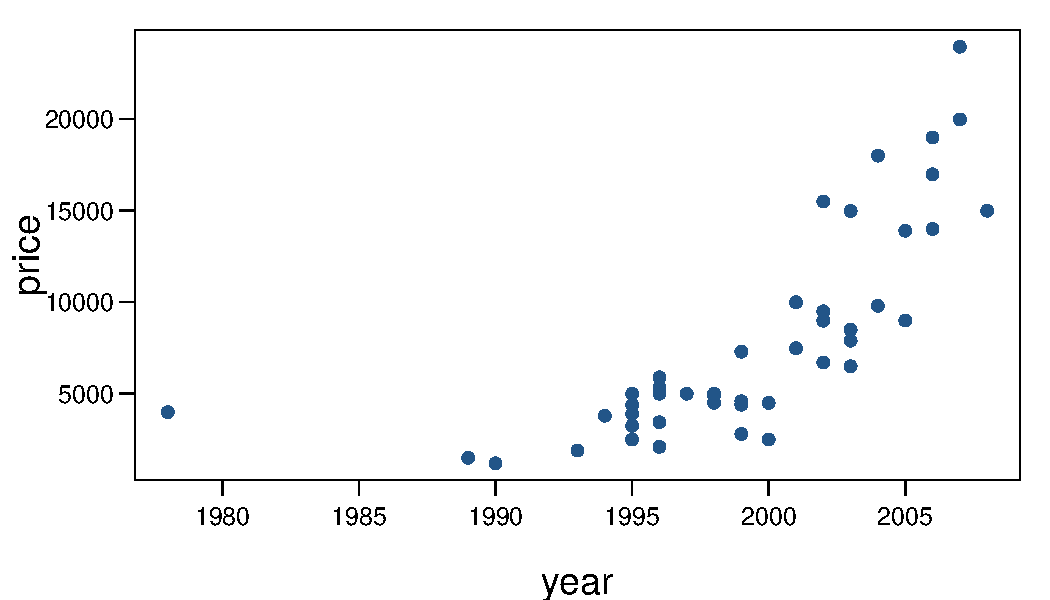
\includegraphics[width=0.7\textwidth]{figures/pickup/pu_price_year_scat_allyrs}
\end{center}

\ct{From: \webURL{http://faculty.chicagobooth.edu/robert.gramacy/teaching.html}}


\end{frame}

%%%%%%%%%%%%%%%%%%%%%%%%%%%%%%%%%%%

\begin{frame}[fragile]
\frametitle{Remove unusual observations}

Let's remove trucks older than 20 years, and only focus on trucks made in 1992 or later.

\pause

\disc{Now what can you say about the relationship?}

\begin{center}
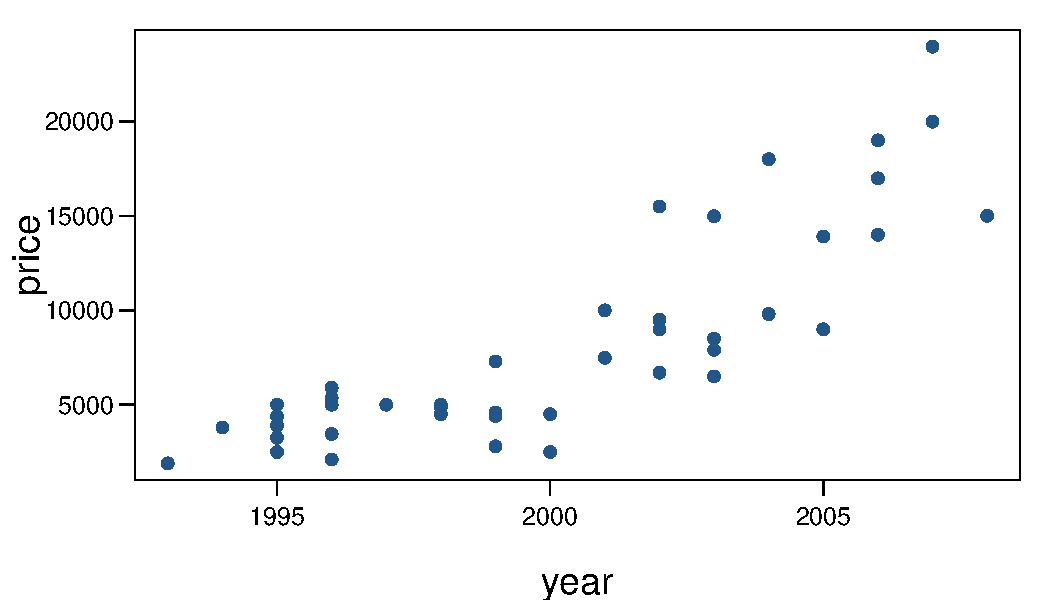
\includegraphics[width=0.7\textwidth]{figures/pickup/pu_price_year_scat_noline}
\end{center}

\end{frame}

%%%%%%%%%%%%%%%%%%%%%%%%%%%%%%%%%%%

\begin{frame}
\frametitle{Truck prices - linear model?}

\vspace{-0.25cm}

\twocol{0.63}{0.35}
{
\begin{center}
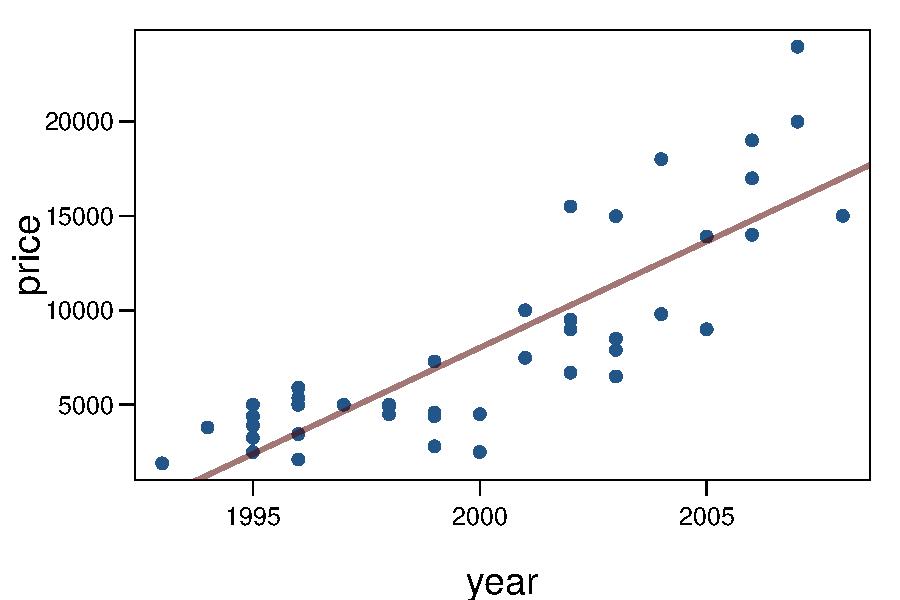
\includegraphics[width=\textwidth]{figures/pickup/pu_price_year_scat} \\
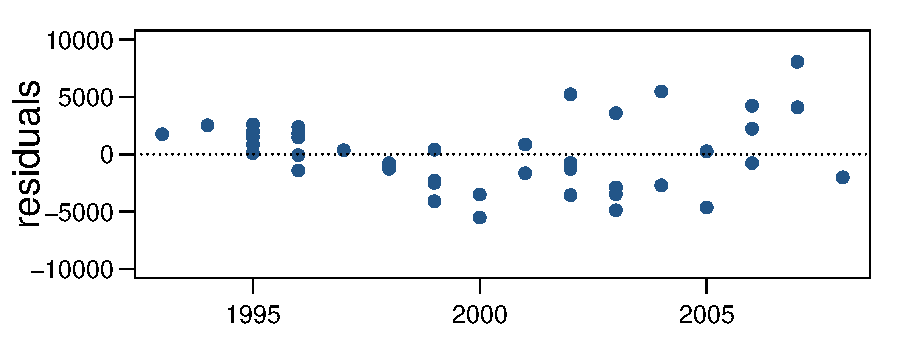
\includegraphics[width=\textwidth]{figures/pickup/pu_price_year_res}
\end{center}
}
{
\hl{Model:} \[ \widehat{price} = b_0 + b_1~year \]
\pause
The linear model doesn't appear to be a good fit since the residuals have non-constant variance. \\
}

\end{frame}

%%%%%%%%%%%%%%%%%%%%%%%%%%%%%%%%%%%

\begin{frame}
\frametitle{Truck prices - log transform of the response variable}

\vspace{-0.25cm}

\twocol{0.63}{0.35}
{
\begin{center}
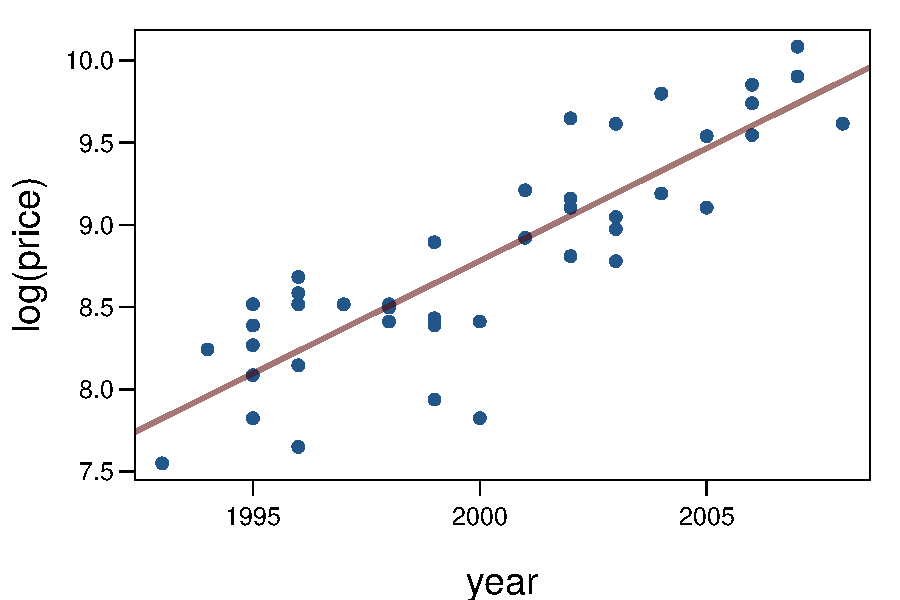
\includegraphics[width=\textwidth]{figures/pickup/pu_price_year_scat_log} \\
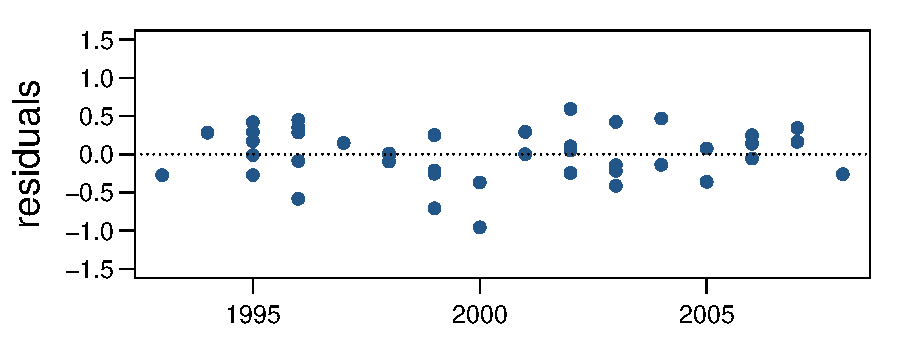
\includegraphics[width=\textwidth]{figures/pickup/pu_price_year_res_log}
\end{center}
}
{
\hl{Model:} \[ \widehat{log(price)} = b_0 + b_1~year \]
\pause
We applied a log transformation to the response variable. The relationship now seems linear, and the residuals no longer have non-constant variance.
}

\end{frame}

%%%%%%%%%%%%%%%%%%%%%%%%%%%%%%%%%%%

\begin{frame}
\frametitle{Interpreting models with log transformation}

\begin{center}
\begin{tabular}{rrrrr}
  \hline
 & Estimate & Std. Error & t value & Pr($>$$|$t$|$) \\ 
  \hline
(Intercept) & -265.07 & 25.04 & -10.59 & 0.00 \\ 
  pu\$year & 0.14 & 0.01 & 10.94 & 0.00 \\ 
   \hline
\end{tabular}
\end{center}

\pause
\[ \hl{\text{Model: }} \widehat{log(price)} = -265.07 + 0.14~year \]

\pause

\begin{itemize}

\item For each additional year the car is newer (for each year decrease in car's age) we would expect the log price of the car to increase on average by 0.14 log dollars.

\pause

\item which is not very useful...

\end{itemize}

\end{frame}

%%%%%%%%%%%%%%%%%%%%%%%%%%%%%%%%%%%

\begin{frame}
\frametitle{Working with logs}

\begin{itemize}

\item Subtraction and logs: $log(a) - log(b) = log(\frac{a}{b})$

\pause

\item Natural logarithm: $e^{log(x)} = x$

\pause

\item We can these identities to ``undo" the log transformation 

\end{itemize}


\end{frame}


%%%%%%%%%%%%%%%%%%%%%%%%%%%%%%%%%%%

\begin{frame}
\frametitle{Interpreting models with log transformation (cont.)}

The slope coefficient for the log transformed model is 0.14, meaning the \underline{log} price difference between cars that are one year apart is predicted to be 0.14 log dollars.

\begin{eqnarray*}
\text{log(price at year $x + 1$)} - \text{log(price at year $x$)} &=& 0.14 \\
\pause
log \pr{ \frac{\text{price at year $x + 1$}}{\text{price at year $x$}} } &=& 0.14 \\
\pause
e^{log \pr{ \frac{\text{price at year $x + 1$}}{\text{price at year $x$}} }} &=& e^{0.14} \\
\pause
\frac{\text{price at year $x + 1$}}{\text{price at year $x$}} &=& 1.15
\end{eqnarray*}

\pause

For each additional year the car is newer (for each year decrease in car's age) we would expect the price of the car to increase on average \red{by a factor of 1.15}.

\end{frame}

%%%%%%%%%%%%%%%%%%%%%%%%%%%%%%%%%%%

\begin{frame}
\frametitle{Recap: dealing with non-constant variance}

\begin{itemize}

\item Non-constant variance is one of the most common model violations, however it is usually fixable by transforming the response ($y$) variable

\pause

\item The most common variance stabilizing transform is the log transformation: $log(y)$, especially useful when the response variable is (extremely) right skewed.

\pause

\item When using a log transformation on the response variable the interpretation of the slope changes: \pause
\begin{itemize}
\item For each unit increase in $x$, y is expected on average to decrease/increase by a factor of $e^{b_1}$.
\end{itemize}

\pause

\item Another useful transformation is the square root: $\sqrt{y}$, especially useful when the response variable is counts.

\pause

\item These transformations may also be useful when the relationship is non-linear, but in those cases a polynomial regression may also be needed.

\end{itemize}

\end{frame}

%%%%%%%%%%%%%%%%%%%%%%%%%%%%%%%%%%%

\section{Case study}

%%%%%%%%%%%%%%%%%%%%%%%%%%%%%%%%%%%

\begin{frame}
\frametitle{}

\app{7.4 Application exercise}{ACS log transform...}

\end{frame}

%%%%%%%%%%%%%%%%%%%%%%%%%%%%%%%%%%%

\end{document}